\documentclass[conference]{IEEEtran}
\usepackage[ngerman]{babel}
\usepackage[utf8]{inputenc}
\usepackage[T1]{fontenc}
\usepackage{graphicx}
\usepackage{caption}
\usepackage{subcaption}

\begin{document}
\title{Verteilte eingebettete Systeme für Netzwerk-Service-Assurance-Tests}
\author{\IEEEauthorblockN{Christian Rebischke}
\IEEEauthorblockA{Technische Universität Clausthal\\
Rechenzentrum\\
Email: Christian.Rebischke@tu-clausthal.de}}

\maketitle

\begin{abstract}
    Um eine gleichbleibende Netzqualität innerhalb des Netzes der
    TU Clausthal zu gewährleisten, werden Einplatinencomputer auf dem
    Campus verteilt, um Service-Assurance-Tests durchzuführen. Diese
    Tests sollen eine gleichbleibende und stabile Verbindung garantieren
    und beim Abweichen von Messergebnissen einen Netzwerkadministrator
    alarmieren. Die Ergebnisse sollen in einer Datenbank gespeichert und
    für die weitere Verwertung gefiltert und optimiert
    werden. Dabei ist geplant, die Masse an Einplatinencomputern mit
    State-of-the-Art-Orchestration und Config-Management-Tools im
    Schwarm zu administrieren. Zusätzlich ist es denkbar, über diese
    verteilten Netzwerkknoten diverse Sicherheitstests im Netzwerk
    durchzuführen wie beispielsweise das Erkennen von ungewünschten
    WLAN-Hotspots oder von Angreifern innerhalb des TU-Netzes.
\end{abstract}

\IEEEpeerreviewmaketitle

\section{Einleitung}
Im Zeitalter immer stärkerer Digitalisierung nimmt ein stabiles und
zuverlässiges Netz eine immer wichtigere Rolle ein. Dies ist gerade im
akademischen Umfeld, in dem Themen wie verteiltes Rechnen eine große
Rolle spielen zu spüren. Abweichungen oder Netzausfälle können in so einem Fall
ganze Berechnungen zu nichte machen. Um ein stabiles Netz zu
gewährleisten gibt es Service-Assurance-Tests. Service-Assurance-Tests
sollen eine bestimmte Service-Qualität zusichern. Dies kann
bei einer Uptime-Garantie anfangen und über eine Bandbreiten-Garantie bis zur
Überwachung von Service-Level-Agreements reichen.
\subsection{Technische Details}
Als Grundlage für die Service-Assurance-Tests sollen
Einplatinencomputer wie beispielsweise der Raspberry Pi oder der Odroid
dienen. Der Vorteil ist ein geringer Preis in der Anschaffung und
eine stabile Basis auf offener Software, die es ermöglicht, das System
beliebig zu erweitern und zu verändern. Als Betriebssystem wird eine auf
Debian oder CentOS basierende Linux-Distribution zum Einsatz kommen. Um
maximale Genauigkeit zu garantieren, ist außerdem ein nativer
1Gigabit-Ethernet-Port vonnöten. Die restlichen Hardware-Anforderungen
sind variabel, aber 20 GB Festplatte in Form eines Flash-Speichers, bis
zu 4 CPU-Kerne und 2\-4 GB RAM sollten ausreichen. Um die veteilten
Einplatinencomputer zentral zu verwalten ist ein modernes
Configuration-Management mit einer Key-Value-Datenbank auf Basis von Hiera
und Puppet geplant. Dafür wird es einen zentralen Puppet-Server geben
von dem aktuelle Konfigurationsdaten mit einem Pull-Mechanismus an die
Clients verteilt werden. Dadurch sind manuelle Arbeiten auf den Clients
nicht mehr nötig. Die von den Clients gewonnenen Daten sollen an eine
zentrale Datenbank weitergeleitet werden. Zur Visualisierung ist eine
Grafana-Instanz geplant.
\begin{figure}[h]
    \centering
    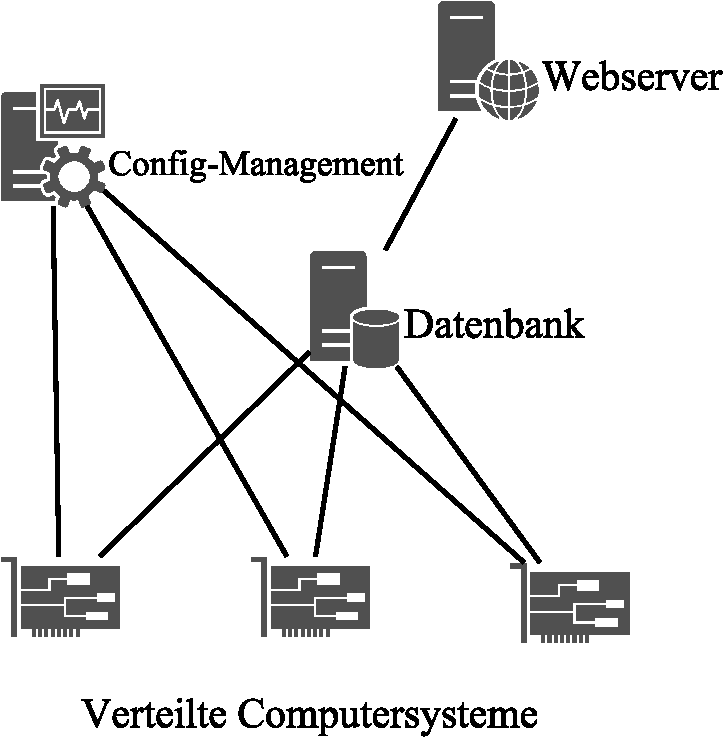
\includegraphics[width=0.5\textwidth]{figures/network.pdf}
    \caption{Netzwerk-Grundriss des Projekts}\label{fig:1}
\end{figure}

\section*{Danksagung}
Ich danke dem Rechenzentrum der TU Clausthal, dass ich dort meine
Bachelor-Arbeit schreiben darf.

\end{document}
